\documentclass[1p]{elsarticle_modified}
%\bibliographystyle{elsarticle-num}

%\usepackage[colorlinks]{hyperref}
%\usepackage{abbrmath_seonhwa} %\Abb, \Ascr, \Acal ,\Abf, \Afrak
\usepackage{amsfonts}
\usepackage{amssymb}
\usepackage{amsmath}
\usepackage{amsthm}
\usepackage{scalefnt}
\usepackage{amsbsy}
\usepackage{kotex}
\usepackage{caption}
\usepackage{subfig}
\usepackage{color}
\usepackage{graphicx}
\usepackage{xcolor} %% white, black, red, green, blue, cyan, magenta, yellow
\usepackage{float}
\usepackage{setspace}
\usepackage{hyperref}

\usepackage{tikz}
\usetikzlibrary{arrows}

\usepackage{multirow}
\usepackage{array} % fixed length table
\usepackage{hhline}

%%%%%%%%%%%%%%%%%%%%%
\makeatletter
\renewcommand*\env@matrix[1][\arraystretch]{%
	\edef\arraystretch{#1}%
	\hskip -\arraycolsep
	\let\@ifnextchar\new@ifnextchar
	\array{*\c@MaxMatrixCols c}}
\makeatother %https://tex.stackexchange.com/questions/14071/how-can-i-increase-the-line-spacing-in-a-matrix
%%%%%%%%%%%%%%%

\usepackage[normalem]{ulem}

\newcommand{\msout}[1]{\ifmmode\text{\sout{\ensuremath{#1}}}\else\sout{#1}\fi}
%SOURCE: \msout is \stkout macro in https://tex.stackexchange.com/questions/20609/strikeout-in-math-mode

\newcommand{\cancel}[1]{
	\ifmmode
	{\color{red}\msout{#1}}
	\else
	{\color{red}\sout{#1}}
	\fi
}

\newcommand{\add}[1]{
	{\color{blue}\uwave{#1}}
}

\newcommand{\replace}[2]{
	\ifmmode
	{\color{red}\msout{#1}}{\color{blue}\uwave{#2}}
	\else
	{\color{red}\sout{#1}}{\color{blue}\uwave{#2}}
	\fi
}

\newcommand{\Sol}{\mathcal{S}} %segment
\newcommand{\D}{D} %diagram
\newcommand{\A}{\mathcal{A}} %arc


%%%%%%%%%%%%%%%%%%%%%%%%%%%%%5 test

\def\sl{\operatorname{\textup{SL}}(2,\Cbb)}
\def\psl{\operatorname{\textup{PSL}}(2,\Cbb)}
\def\quan{\mkern 1mu \triangleright \mkern 1mu}

\theoremstyle{definition}
\newtheorem{thm}{Theorem}[section]
\newtheorem{prop}[thm]{Proposition}
\newtheorem{lem}[thm]{Lemma}
\newtheorem{ques}[thm]{Question}
\newtheorem{cor}[thm]{Corollary}
\newtheorem{defn}[thm]{Definition}
\newtheorem{exam}[thm]{Example}
\newtheorem{rmk}[thm]{Remark}
\newtheorem{alg}[thm]{Algorithm}

\newcommand{\I}{\sqrt{-1}}
\begin{document}

%\begin{frontmatter}
%
%\title{Boundary parabolic representations of knots up to 8 crossings}
%
%%% Group authors per affiliation:
%\author{Yunhi Cho} 
%\address{Department of Mathematics, University of Seoul, Seoul, Korea}
%\ead{yhcho@uos.ac.kr}
%
%
%\author{Seonhwa Kim} %\fnref{s_kim}}
%\address{Center for Geometry and Physics, Institute for Basic Science, Pohang, 37673, Korea}
%\ead{ryeona17@ibs.re.kr}
%
%\author{Hyuk Kim}
%\address{Department of Mathematical Sciences, Seoul National University, Seoul 08826, Korea}
%\ead{hyukkim@snu.ac.kr}
%
%\author{Seokbeom Yoon}
%\address{Department of Mathematical Sciences, Seoul National University, Seoul, 08826,  Korea}
%\ead{sbyoon15@snu.ac.kr}
%
%\begin{abstract}
%We find all boundary parabolic representation of knots up to 8 crossings.
%
%\end{abstract}
%\begin{keyword}
%    \MSC[2010] 57M25 
%\end{keyword}
%
%\end{frontmatter}

%\linenumbers
%\tableofcontents
%
\newcommand\colored[1]{\textcolor{white}{\rule[-0.35ex]{0.8em}{1.4ex}}\kern-0.8em\color{red} #1}%
%\newcommand\colored[1]{\textcolor{white}{ #1}\kern-2.17ex	\textcolor{white}{ #1}\kern-1.81ex	\textcolor{white}{ #1}\kern-2.15ex\color{red}#1	}

{\Large $\underline{12a_{0627}~(K12a_{0627})}$}

\setlength{\tabcolsep}{10pt}
\renewcommand{\arraystretch}{1.6}
\vspace{1cm}\begin{tabular}{m{100pt}>{\centering\arraybackslash}m{274pt}}
\multirow{5}{120pt}{
	\centering
	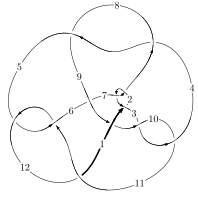
\includegraphics[width=112pt]{../../../GIT/diagram.site/Diagrams/png/1428_12a_0627.png}\\
\ \ \ A knot diagram\footnotemark}&
\allowdisplaybreaks
\textbf{Linearized knot diagam} \\
\cline{2-2}
 &
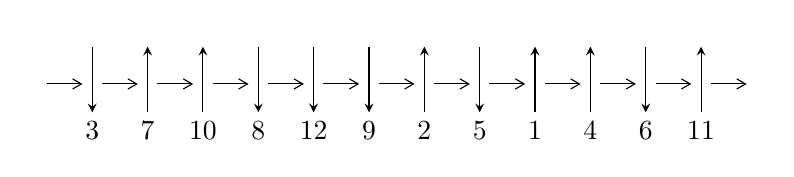
\begin{tikzpicture}[x=20pt, y=17pt]
	% nodes
	\node (C0) at (0, 0) {};
	\node (C1) at (1, 0) {};
	\node (C1U) at (1, +1) {};
	\node (C1D) at (1, -1) {3};

	\node (C2) at (2, 0) {};
	\node (C2U) at (2, +1) {};
	\node (C2D) at (2, -1) {7};

	\node (C3) at (3, 0) {};
	\node (C3U) at (3, +1) {};
	\node (C3D) at (3, -1) {10};

	\node (C4) at (4, 0) {};
	\node (C4U) at (4, +1) {};
	\node (C4D) at (4, -1) {8};

	\node (C5) at (5, 0) {};
	\node (C5U) at (5, +1) {};
	\node (C5D) at (5, -1) {12};

	\node (C6) at (6, 0) {};
	\node (C6U) at (6, +1) {};
	\node (C6D) at (6, -1) {9};

	\node (C7) at (7, 0) {};
	\node (C7U) at (7, +1) {};
	\node (C7D) at (7, -1) {2};

	\node (C8) at (8, 0) {};
	\node (C8U) at (8, +1) {};
	\node (C8D) at (8, -1) {5};

	\node (C9) at (9, 0) {};
	\node (C9U) at (9, +1) {};
	\node (C9D) at (9, -1) {1};

	\node (C10) at (10, 0) {};
	\node (C10U) at (10, +1) {};
	\node (C10D) at (10, -1) {4};

	\node (C11) at (11, 0) {};
	\node (C11U) at (11, +1) {};
	\node (C11D) at (11, -1) {6};

	\node (C12) at (12, 0) {};
	\node (C12U) at (12, +1) {};
	\node (C12D) at (12, -1) {11};
	\node (C13) at (13, 0) {};

	% arrows
	\draw[->,>={angle 60}]
	(C0) edge (C1) (C1) edge (C2) (C2) edge (C3) (C3) edge (C4) (C4) edge (C5) (C5) edge (C6) (C6) edge (C7) (C7) edge (C8) (C8) edge (C9) (C9) edge (C10) (C10) edge (C11) (C11) edge (C12) (C12) edge (C13) ;	\draw[->,>=stealth]
	(C1U) edge (C1D) (C2D) edge (C2U) (C3D) edge (C3U) (C4U) edge (C4D) (C5U) edge (C5D) (C6U) edge (C6D) (C7D) edge (C7U) (C8U) edge (C8D) (C9D) edge (C9U) (C10D) edge (C10U) (C11U) edge (C11D) (C12D) edge (C12U) ;
	\end{tikzpicture} \\
\hhline{~~} \\& 
\textbf{Solving Sequence} \\ \cline{2-2} 
 &
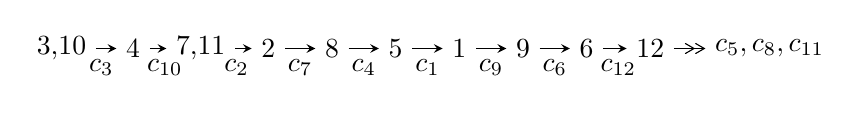
\begin{tikzpicture}[x=23pt, y=7pt]
	% node
	\node (A0) at (-1/8, 0) {3,10};
	\node (A1) at (1, 0) {4};
	\node (A2) at (33/16, 0) {7,11};
	\node (A3) at (25/8, 0) {2};
	\node (A4) at (33/8, 0) {8};
	\node (A5) at (41/8, 0) {5};
	\node (A6) at (49/8, 0) {1};
	\node (A7) at (57/8, 0) {9};
	\node (A8) at (65/8, 0) {6};
	\node (A9) at (73/8, 0) {12};
	\node (C1) at (1/2, -1) {$c_{3}$};
	\node (C2) at (3/2, -1) {$c_{10}$};
	\node (C3) at (21/8, -1) {$c_{2}$};
	\node (C4) at (29/8, -1) {$c_{7}$};
	\node (C5) at (37/8, -1) {$c_{4}$};
	\node (C6) at (45/8, -1) {$c_{1}$};
	\node (C7) at (53/8, -1) {$c_{9}$};
	\node (C8) at (61/8, -1) {$c_{6}$};
	\node (C9) at (69/8, -1) {$c_{12}$};
	\node (A10) at (11, 0) {$c_{5},c_{8},c_{11}$};

	% edge
	\draw[->,>=stealth]	
	(A0) edge (A1) (A1) edge (A2) (A2) edge (A3) (A3) edge (A4) (A4) edge (A5) (A5) edge (A6) (A6) edge (A7) (A7) edge (A8) (A8) edge (A9) ;
	\draw[->>,>={angle 60}]	
	(A9) edge (A10);
\end{tikzpicture} \\ 

\end{tabular} \\

\footnotetext{
The image of knot diagram is generated by the software ``\textbf{Draw programme}" developed by Andrew Bartholomew(\url{http://www.layer8.co.uk/maths/draw/index.htm\#Running-draw}), where we modified some parts for our purpose(\url{https://github.com/CATsTAILs/LinksPainter}).
}\phantom \\ \newline 
\centering \textbf{Ideals for irreducible components\footnotemark of $X_{\text{par}}$} 
 
\begin{align*}
I^u_{1}&=\langle 
6.74702\times10^{811} u^{141}+1.09442\times10^{812} u^{140}+\cdots+3.41875\times10^{813} b-2.08476\times10^{815},\\
\phantom{I^u_{1}}&\phantom{= \langle  }1.09226\times10^{816} u^{141}+1.97778\times10^{816} u^{140}+\cdots+7.17596\times10^{816} a-4.28834\times10^{819},\\
\phantom{I^u_{1}}&\phantom{= \langle  }u^{142}+u^{141}+\cdots-907109 u+2099\rangle \\
I^u_{2}&=\langle 
1264191898 u^{27}+4324326347 u^{26}+\cdots+52008813 b+2153585138,\\
\phantom{I^u_{2}}&\phantom{= \langle  }2700862307 u^{27}+9574821553 u^{26}+\cdots+52008813 a+5465518489,\;u^{28}+4 u^{27}+\cdots+4 u+1\rangle \\
\\
\end{align*}
\raggedright * 2 irreducible components of $\dim_{\mathbb{C}}=0$, with total 170 representations.\\
\footnotetext{All coefficients of polynomials are rational numbers. But the coefficients are sometimes approximated in decimal forms when there is not enough margin.}
\newpage
\renewcommand{\arraystretch}{1}
\centering \section*{I. $I^u_{1}= \langle 6.75\times10^{811} u^{141}+1.09\times10^{812} u^{140}+\cdots+3.42\times10^{813} b-2.08\times10^{815},\;1.09\times10^{816} u^{141}+1.98\times10^{816} u^{140}+\cdots+7.18\times10^{816} a-4.29\times10^{819},\;u^{142}+u^{141}+\cdots-907109 u+2099 \rangle$}
\flushleft \textbf{(i) Arc colorings}\\
\begin{tabular}{m{7pt} m{180pt} m{7pt} m{180pt} }
\flushright $a_{3}=$&$\begin{pmatrix}1\\0\end{pmatrix}$ \\
\flushright $a_{10}=$&$\begin{pmatrix}0\\u\end{pmatrix}$ \\
\flushright $a_{4}=$&$\begin{pmatrix}1\\- u^2\end{pmatrix}$ \\
\flushright $a_{7}=$&$\begin{pmatrix}-0.152212 u^{141}-0.275612 u^{140}+\cdots-167326. u+597.599\\-0.0197353 u^{141}-0.0320124 u^{140}+\cdots-26578.0 u+60.9802\end{pmatrix}$ \\
\flushright $a_{11}=$&$\begin{pmatrix}u\\- u^3+u\end{pmatrix}$ \\
\flushright $a_{2}=$&$\begin{pmatrix}0.125998 u^{141}+0.225405 u^{140}+\cdots+139852. u-473.200\\0.0772454 u^{141}+0.149742 u^{140}+\cdots+75128.4 u-173.760\end{pmatrix}$ \\
\flushright $a_{8}=$&$\begin{pmatrix}-0.119370 u^{141}-0.218578 u^{140}+\cdots-127989. u+612.605\\-0.0471017 u^{141}-0.0899098 u^{140}+\cdots-46092.1 u+105.834\end{pmatrix}$ \\
\flushright $a_{5}=$&$\begin{pmatrix}-0.297171 u^{141}-0.547343 u^{140}+\cdots-316063. u+393.790\\-0.0689418 u^{141}-0.131837 u^{140}+\cdots-69332.9 u+162.006\end{pmatrix}$ \\
\flushright $a_{1}=$&$\begin{pmatrix}0.203243 u^{141}+0.375147 u^{140}+\cdots+214980. u-646.960\\0.0772454 u^{141}+0.149742 u^{140}+\cdots+75128.4 u-173.760\end{pmatrix}$ \\
\flushright $a_{9}=$&$\begin{pmatrix}0.355590 u^{141}+0.673424 u^{140}+\cdots+358791. u-883.101\\0.175090 u^{141}+0.317526 u^{140}+\cdots+193670. u-449.231\end{pmatrix}$ \\
\flushright $a_{6}=$&$\begin{pmatrix}0.166507 u^{141}+0.296018 u^{140}+\cdots+191000. u-190.579\\0.110343 u^{141}+0.205179 u^{140}+\cdots+116314. u-270.736\end{pmatrix}$ \\
\flushright $a_{12}=$&$\begin{pmatrix}0.179184 u^{141}+0.325133 u^{140}+\cdots+194744. u-600.039\\0.0802693 u^{141}+0.155031 u^{140}+\cdots+78385.4 u-181.319\end{pmatrix}$\\&\end{tabular}
\flushleft \textbf{(ii) Obstruction class $= -1$}\\~\\
\flushleft \textbf{(iii) Cusp Shapes $= -0.0416421 u^{141}-0.0832729 u^{140}+\cdots-41293.2 u+89.3667$}\\~\\
\newpage\renewcommand{\arraystretch}{1}
\flushleft \textbf{(iv) u-Polynomials at the component}\newline \\
\begin{tabular}{m{50pt}|m{274pt}}
Crossings & \hspace{64pt}u-Polynomials at each crossing \\
\hline $$\begin{aligned}c_{1}\end{aligned}$$&$\begin{aligned}
&9(9 u^{142}+519 u^{141}+\cdots+57707 u+5329)
\end{aligned}$\\
\hline $$\begin{aligned}c_{2},c_{7}\end{aligned}$$&$\begin{aligned}
&3(3 u^{142}+3 u^{141}+\cdots+359 u-73)
\end{aligned}$\\
\hline $$\begin{aligned}c_{3},c_{10}\end{aligned}$$&$\begin{aligned}
&u^{142}+u^{141}+\cdots-907109 u+2099
\end{aligned}$\\
\hline $$\begin{aligned}c_{4},c_{8}\end{aligned}$$&$\begin{aligned}
&u^{142}- u^{141}+\cdots+907109 u+2099
\end{aligned}$\\
\hline $$\begin{aligned}c_{5},c_{11}\end{aligned}$$&$\begin{aligned}
&3(3 u^{142}-3 u^{141}+\cdots-359 u-73)
\end{aligned}$\\
\hline $$\begin{aligned}c_{6}\end{aligned}$$&$\begin{aligned}
&u^{142}-4 u^{141}+\cdots+76091739 u-4428063
\end{aligned}$\\
\hline $$\begin{aligned}c_{9}\end{aligned}$$&$\begin{aligned}
&u^{142}+4 u^{141}+\cdots-76091739 u-4428063
\end{aligned}$\\
\hline $$\begin{aligned}c_{12}\end{aligned}$$&$\begin{aligned}
&9(9 u^{142}-519 u^{141}+\cdots-57707 u+5329)
\end{aligned}$\\
\hline
\end{tabular}\\~\\
\newpage\renewcommand{\arraystretch}{1}
\flushleft \textbf{(v) Riley Polynomials at the component}\newline \\
\begin{tabular}{m{50pt}|m{274pt}}
Crossings & \hspace{64pt}Riley Polynomials at each crossing \\
\hline $$\begin{aligned}c_{1},c_{12}\end{aligned}$$&$\begin{aligned}
&81(81 y^{142}+6327 y^{141}+\cdots-2.56016\times10^{9} y+2.83982\times10^{7})
\end{aligned}$\\
\hline $$\begin{aligned}c_{2},c_{5},c_{7}\\c_{11}\end{aligned}$$&$\begin{aligned}
&9(9 y^{142}+519 y^{141}+\cdots+57707 y+5329)
\end{aligned}$\\
\hline $$\begin{aligned}c_{3},c_{4},c_{8}\\c_{10}\end{aligned}$$&$\begin{aligned}
&y^{142}-93 y^{141}+\cdots-823753833325 y+4405801
\end{aligned}$\\
\hline $$\begin{aligned}c_{6},c_{9}\end{aligned}$$&$\begin{aligned}
&y^{142}-26 y^{141}+\cdots-783996286987719 y+19607741931969
\end{aligned}$\\
\hline
\end{tabular}\\~\\
\newpage\flushleft \textbf{(vi) Complex Volumes and Cusp Shapes}
$$\begin{array}{c|c|c}  
\text{Solutions to }I^u_{1}& \I (\text{vol} + \sqrt{-1}CS) & \text{Cusp shape}\\
 \hline 
\begin{aligned}
u &= \phantom{-}0.999777 + 0.091981 I \\
a &= \phantom{-}1.75501 + 0.96204 I \\
b &= -1.11776 - 1.04446 I\end{aligned}
 & \phantom{-}0.115587 + 0.315701 I & \phantom{-0.000000 } 0 \\ \hline\begin{aligned}
u &= \phantom{-}0.999777 - 0.091981 I \\
a &= \phantom{-}1.75501 - 0.96204 I \\
b &= -1.11776 + 1.04446 I\end{aligned}
 & \phantom{-}0.115587 - 0.315701 I & \phantom{-0.000000 } 0 \\ \hline\begin{aligned}
u &= \phantom{-}0.972850 + 0.179673 I \\
a &= \phantom{-}0.737834 + 0.307202 I \\
b &= -0.132900 + 1.074160 I\end{aligned}
 & \phantom{-}1.78140 + 1.19765 I & \phantom{-0.000000 } 0 \\ \hline\begin{aligned}
u &= \phantom{-}0.972850 - 0.179673 I \\
a &= \phantom{-}0.737834 - 0.307202 I \\
b &= -0.132900 - 1.074160 I\end{aligned}
 & \phantom{-}1.78140 - 1.19765 I & \phantom{-0.000000 } 0 \\ \hline\begin{aligned}
u &= \phantom{-}0.097398 + 0.982037 I \\
a &= \phantom{-}0.851382 - 0.422463 I \\
b &= -0.698611 - 0.418753 I\end{aligned}
 & -3.66799 - 2.04886 I & \phantom{-0.000000 } 0 \\ \hline\begin{aligned}
u &= \phantom{-}0.097398 - 0.982037 I \\
a &= \phantom{-}0.851382 + 0.422463 I \\
b &= -0.698611 + 0.418753 I\end{aligned}
 & -3.66799 + 2.04886 I & \phantom{-0.000000 } 0 \\ \hline\begin{aligned}
u &= \phantom{-}0.891887 + 0.409098 I \\
a &= -0.266032 - 0.098205 I \\
b &= \phantom{-}0.688939 + 0.119170 I\end{aligned}
 & -0.62703 - 2.36846 I & \phantom{-0.000000 } 0 \\ \hline\begin{aligned}
u &= \phantom{-}0.891887 - 0.409098 I \\
a &= -0.266032 + 0.098205 I \\
b &= \phantom{-}0.688939 - 0.119170 I\end{aligned}
 & -0.62703 + 2.36846 I & \phantom{-0.000000 } 0 \\ \hline\begin{aligned}
u &= -0.582706 + 0.835940 I \\
a &= \phantom{-}1.115760 + 0.211551 I \\
b &= -0.134406 + 1.156220 I\end{aligned}
 & -8.51460 - 0.20375 I & \phantom{-0.000000 } 0 \\ \hline\begin{aligned}
u &= -0.582706 - 0.835940 I \\
a &= \phantom{-}1.115760 - 0.211551 I \\
b &= -0.134406 - 1.156220 I\end{aligned}
 & -8.51460 + 0.20375 I & \phantom{-0.000000 } 0\\
 \hline 
 \end{array}$$\newpage$$\begin{array}{c|c|c}  
\text{Solutions to }I^u_{1}& \I (\text{vol} + \sqrt{-1}CS) & \text{Cusp shape}\\
 \hline 
\begin{aligned}
u &= -0.735906 + 0.603682 I \\
a &= -0.535807 - 1.237880 I \\
b &= \phantom{-}0.377524 - 1.068500 I\end{aligned}
 & -4.03516 - 0.96934 I & \phantom{-0.000000 } 0 \\ \hline\begin{aligned}
u &= -0.735906 - 0.603682 I \\
a &= -0.535807 + 1.237880 I \\
b &= \phantom{-}0.377524 + 1.068500 I\end{aligned}
 & -4.03516 + 0.96934 I & \phantom{-0.000000 } 0 \\ \hline\begin{aligned}
u &= \phantom{-}0.941778 + 0.066068 I \\
a &= -1.86453 + 0.81269 I \\
b &= \phantom{-}1.10557 - 1.08573 I\end{aligned}
 & -0.115587 + 0.315701 I & \phantom{-0.000000 } 0 \\ \hline\begin{aligned}
u &= \phantom{-}0.941778 - 0.066068 I \\
a &= -1.86453 - 0.81269 I \\
b &= \phantom{-}1.10557 + 1.08573 I\end{aligned}
 & -0.115587 - 0.315701 I & \phantom{-0.000000 } 0 \\ \hline\begin{aligned}
u &= -1.023860 + 0.260578 I \\
a &= \phantom{-}2.78417 - 1.34157 I \\
b &= -0.534031 + 0.941701 I\end{aligned}
 & -2.54184 - 8.91574 I & \phantom{-0.000000 } 0 \\ \hline\begin{aligned}
u &= -1.023860 - 0.260578 I \\
a &= \phantom{-}2.78417 + 1.34157 I \\
b &= -0.534031 - 0.941701 I\end{aligned}
 & -2.54184 + 8.91574 I & \phantom{-0.000000 } 0 \\ \hline\begin{aligned}
u &= \phantom{-}1.048170 + 0.152717 I \\
a &= -2.23658 - 1.78317 I \\
b &= \phantom{-}0.526778 + 0.924900 I\end{aligned}
 & -3.02313 + 3.31558 I & \phantom{-0.000000 } 0 \\ \hline\begin{aligned}
u &= \phantom{-}1.048170 - 0.152717 I \\
a &= -2.23658 + 1.78317 I \\
b &= \phantom{-}0.526778 - 0.924900 I\end{aligned}
 & -3.02313 - 3.31558 I & \phantom{-0.000000 } 0 \\ \hline\begin{aligned}
u &= \phantom{-}0.907559 + 0.556741 I \\
a &= \phantom{-}1.026920 + 0.235437 I \\
b &= \phantom{-}0.395468 - 0.905996 I\end{aligned}
 & -3.81941 - 1.48950 I & \phantom{-0.000000 } 0 \\ \hline\begin{aligned}
u &= \phantom{-}0.907559 - 0.556741 I \\
a &= \phantom{-}1.026920 - 0.235437 I \\
b &= \phantom{-}0.395468 + 0.905996 I\end{aligned}
 & -3.81941 + 1.48950 I & \phantom{-0.000000 } 0\\
 \hline 
 \end{array}$$\newpage$$\begin{array}{c|c|c}  
\text{Solutions to }I^u_{1}& \I (\text{vol} + \sqrt{-1}CS) & \text{Cusp shape}\\
 \hline 
\begin{aligned}
u &= -0.969830 + 0.440655 I \\
a &= -0.527831 - 0.710169 I \\
b &= -0.141735 - 0.979176 I\end{aligned}
 & -1.16877 - 1.23928 I & \phantom{-0.000000 } 0 \\ \hline\begin{aligned}
u &= -0.969830 - 0.440655 I \\
a &= -0.527831 + 0.710169 I \\
b &= -0.141735 + 0.979176 I\end{aligned}
 & -1.16877 + 1.23928 I & \phantom{-0.000000 } 0 \\ \hline\begin{aligned}
u &= \phantom{-}0.533762 + 0.926281 I \\
a &= -1.215540 + 0.292203 I \\
b &= \phantom{-}0.117807 + 1.109140 I\end{aligned}
 & -7.00419 - 5.60834 I & \phantom{-0.000000 } 0 \\ \hline\begin{aligned}
u &= \phantom{-}0.533762 - 0.926281 I \\
a &= -1.215540 - 0.292203 I \\
b &= \phantom{-}0.117807 - 1.109140 I\end{aligned}
 & -7.00419 + 5.60834 I & \phantom{-0.000000 } 0 \\ \hline\begin{aligned}
u &= -1.047440 + 0.220766 I \\
a &= \phantom{-}0.260757 - 0.045770 I \\
b &= -0.726111 + 0.058471 I\end{aligned}
 & -0.78723 - 1.84537 I & \phantom{-0.000000 } 0 \\ \hline\begin{aligned}
u &= -1.047440 - 0.220766 I \\
a &= \phantom{-}0.260757 + 0.045770 I \\
b &= -0.726111 - 0.058471 I\end{aligned}
 & -0.78723 + 1.84537 I & \phantom{-0.000000 } 0 \\ \hline\begin{aligned}
u &= \phantom{-}0.822605 + 0.424676 I \\
a &= \phantom{-}0.506086 - 1.249620 I \\
b &= -0.395425 - 1.116900 I\end{aligned}
 & -4.23196 + 5.58061 I & \phantom{-0.000000 } 0 \\ \hline\begin{aligned}
u &= \phantom{-}0.822605 - 0.424676 I \\
a &= \phantom{-}0.506086 + 1.249620 I \\
b &= -0.395425 + 1.116900 I\end{aligned}
 & -4.23196 - 5.58061 I & \phantom{-0.000000 } 0 \\ \hline\begin{aligned}
u &= \phantom{-}1.07901\phantom{ +0.000000I} \\
a &= -0.941451\phantom{ +0.000000I} \\
b &= \phantom{-}0.586362\phantom{ +0.000000I}\end{aligned}
 & \phantom{-}1.80252\phantom{ +0.000000I} & \phantom{-0.000000 } 0 \\ \hline\begin{aligned}
u &= -0.891486 + 0.610218 I \\
a &= -1.014450 - 0.251121 I \\
b &= -0.358713 - 0.930244 I\end{aligned}
 & -3.57928 - 3.82983 I & \phantom{-0.000000 } 0\\
 \hline 
 \end{array}$$\newpage$$\begin{array}{c|c|c}  
\text{Solutions to }I^u_{1}& \I (\text{vol} + \sqrt{-1}CS) & \text{Cusp shape}\\
 \hline 
\begin{aligned}
u &= -0.891486 - 0.610218 I \\
a &= -1.014450 + 0.251121 I \\
b &= -0.358713 + 0.930244 I\end{aligned}
 & -3.57928 + 3.82983 I & \phantom{-0.000000 } 0 \\ \hline\begin{aligned}
u &= -0.954768 + 0.543815 I \\
a &= \phantom{-}0.518706 - 0.032264 I \\
b &= -0.091462 + 1.324820 I\end{aligned}
 & -7.29435 - 4.89384 I & \phantom{-0.000000 } 0 \\ \hline\begin{aligned}
u &= -0.954768 - 0.543815 I \\
a &= \phantom{-}0.518706 + 0.032264 I \\
b &= -0.091462 - 1.324820 I\end{aligned}
 & -7.29435 + 4.89384 I & \phantom{-0.000000 } 0 \\ \hline\begin{aligned}
u &= -1.089670 + 0.209938 I \\
a &= -1.36098 + 0.43540 I \\
b &= \phantom{-}1.083980 - 0.532524 I\end{aligned}
 & \phantom{-}1.86233 - 7.66979 I & \phantom{-0.000000 } 0 \\ \hline\begin{aligned}
u &= -1.089670 - 0.209938 I \\
a &= -1.36098 - 0.43540 I \\
b &= \phantom{-}1.083980 + 0.532524 I\end{aligned}
 & \phantom{-}1.86233 + 7.66979 I & \phantom{-0.000000 } 0 \\ \hline\begin{aligned}
u &= \phantom{-}0.504350 + 0.727388 I \\
a &= -0.828417 - 1.023530 I \\
b &= -0.226989 - 0.419380 I\end{aligned}
 & -2.24649 + 6.43121 I & \phantom{-0.000000 } 0 \\ \hline\begin{aligned}
u &= \phantom{-}0.504350 - 0.727388 I \\
a &= -0.828417 + 1.023530 I \\
b &= -0.226989 + 0.419380 I\end{aligned}
 & -2.24649 - 6.43121 I & \phantom{-0.000000 } 0 \\ \hline\begin{aligned}
u &= \phantom{-}0.216819 + 0.829790 I \\
a &= \phantom{-}0.284915 - 0.194348 I \\
b &= -0.614612 + 0.638726 I\end{aligned}
 & \phantom{-}0.90427 + 2.58836 I & \phantom{-0.000000 } 0 \\ \hline\begin{aligned}
u &= \phantom{-}0.216819 - 0.829790 I \\
a &= \phantom{-}0.284915 + 0.194348 I \\
b &= -0.614612 - 0.638726 I\end{aligned}
 & \phantom{-}0.90427 - 2.58836 I & \phantom{-0.000000 } 0 \\ \hline\begin{aligned}
u &= \phantom{-}0.846878 + 0.049904 I \\
a &= \phantom{-}0.69761 + 1.28112 I \\
b &= -0.438756 + 1.143830 I\end{aligned}
 & -3.95688 - 2.31810 I & \phantom{-0.000000 } 0\\
 \hline 
 \end{array}$$\newpage$$\begin{array}{c|c|c}  
\text{Solutions to }I^u_{1}& \I (\text{vol} + \sqrt{-1}CS) & \text{Cusp shape}\\
 \hline 
\begin{aligned}
u &= \phantom{-}0.846878 - 0.049904 I \\
a &= \phantom{-}0.69761 - 1.28112 I \\
b &= -0.438756 - 1.143830 I\end{aligned}
 & -3.95688 + 2.31810 I & \phantom{-0.000000 } 0 \\ \hline\begin{aligned}
u &= -0.846164 + 0.050634 I \\
a &= -3.58337 + 0.37080 I \\
b &= \phantom{-}0.495605 - 0.781614 I\end{aligned}
 & -2.52732 - 0.86075 I & \phantom{-0.000000 } 0 \\ \hline\begin{aligned}
u &= -0.846164 - 0.050634 I \\
a &= -3.58337 - 0.37080 I \\
b &= \phantom{-}0.495605 + 0.781614 I\end{aligned}
 & -2.52732 + 0.86075 I & \phantom{-0.000000 } 0 \\ \hline\begin{aligned}
u &= \phantom{-}1.126400 + 0.264868 I \\
a &= \phantom{-}0.491028 - 0.645301 I \\
b &= \phantom{-}0.081994 - 1.072770 I\end{aligned}
 & \phantom{-}0.22187 + 5.50655 I & \phantom{-0.000000 } 0 \\ \hline\begin{aligned}
u &= \phantom{-}1.126400 - 0.264868 I \\
a &= \phantom{-}0.491028 + 0.645301 I \\
b &= \phantom{-}0.081994 + 1.072770 I\end{aligned}
 & \phantom{-}0.22187 - 5.50655 I & \phantom{-0.000000 } 0 \\ \hline\begin{aligned}
u &= -0.046758 + 0.837944 I \\
a &= \phantom{-}0.95887 + 1.13130 I \\
b &= -0.617919 + 0.954869 I\end{aligned}
 & \phantom{-0.000000 } -7.46414 I & \phantom{-0.000000 } 0 \\ \hline\begin{aligned}
u &= -0.046758 - 0.837944 I \\
a &= \phantom{-}0.95887 - 1.13130 I \\
b &= -0.617919 - 0.954869 I\end{aligned}
 & \phantom{-0.000000 -}7.46414 I & \phantom{-0.000000 } 0 \\ \hline\begin{aligned}
u &= \phantom{-}0.831672 + 0.063981 I \\
a &= \phantom{-}3.53082 - 1.42335 I \\
b &= -0.496555 + 0.758778 I\end{aligned}
 & -1.91137 + 4.69879 I & \phantom{-0.000000 } 0 \\ \hline\begin{aligned}
u &= \phantom{-}0.831672 - 0.063981 I \\
a &= \phantom{-}3.53082 + 1.42335 I \\
b &= -0.496555 - 0.758778 I\end{aligned}
 & -1.91137 - 4.69879 I & \phantom{-0.000000 } 0 \\ \hline\begin{aligned}
u &= \phantom{-}0.608207 + 0.552772 I \\
a &= -0.581035 - 0.562360 I \\
b &= \phantom{-}0.277435 - 0.078683 I\end{aligned}
 & \phantom{-}1.21657 + 1.49421 I & \phantom{-0.000000 } 0\\
 \hline 
 \end{array}$$\newpage$$\begin{array}{c|c|c}  
\text{Solutions to }I^u_{1}& \I (\text{vol} + \sqrt{-1}CS) & \text{Cusp shape}\\
 \hline 
\begin{aligned}
u &= \phantom{-}0.608207 - 0.552772 I \\
a &= -0.581035 + 0.562360 I \\
b &= \phantom{-}0.277435 + 0.078683 I\end{aligned}
 & \phantom{-}1.21657 - 1.49421 I & \phantom{-0.000000 } 0 \\ \hline\begin{aligned}
u &= -0.501974 + 0.645385 I \\
a &= \phantom{-}0.61974 - 1.42878 I \\
b &= \phantom{-}0.203287 - 0.572937 I\end{aligned}
 & -3.03156 - 1.29600 I & \phantom{-0.000000 } 0 \\ \hline\begin{aligned}
u &= -0.501974 - 0.645385 I \\
a &= \phantom{-}0.61974 + 1.42878 I \\
b &= \phantom{-}0.203287 + 0.572937 I\end{aligned}
 & -3.03156 + 1.29600 I & \phantom{-0.000000 } 0 \\ \hline\begin{aligned}
u &= -0.710613 + 0.386852 I \\
a &= -0.527263 - 0.920020 I \\
b &= -0.036444 - 0.874568 I\end{aligned}
 & -1.21657 - 1.49421 I & \phantom{-0.000000 } 0 \\ \hline\begin{aligned}
u &= -0.710613 - 0.386852 I \\
a &= -0.527263 + 0.920020 I \\
b &= -0.036444 + 0.874568 I\end{aligned}
 & -1.21657 + 1.49421 I & \phantom{-0.000000 } 0 \\ \hline\begin{aligned}
u &= -1.158390 + 0.322284 I \\
a &= -1.81306 + 0.42467 I \\
b &= \phantom{-}0.762237 - 1.171010 I\end{aligned}
 & -1.86233 - 7.66979 I & \phantom{-0.000000 } 0 \\ \hline\begin{aligned}
u &= -1.158390 - 0.322284 I \\
a &= -1.81306 - 0.42467 I \\
b &= \phantom{-}0.762237 + 1.171010 I\end{aligned}
 & -1.86233 + 7.66979 I & \phantom{-0.000000 } 0 \\ \hline\begin{aligned}
u &= -0.138862 + 0.779993 I \\
a &= -0.745625 + 0.918804 I \\
b &= \phantom{-}0.560504 + 0.944303 I\end{aligned}
 & -0.90427 + 2.58836 I & \phantom{-0.000000 } 0 \\ \hline\begin{aligned}
u &= -0.138862 - 0.779993 I \\
a &= -0.745625 - 0.918804 I \\
b &= \phantom{-}0.560504 - 0.944303 I\end{aligned}
 & -0.90427 - 2.58836 I & \phantom{-0.000000 } 0 \\ \hline\begin{aligned}
u &= -0.015459 + 1.212910 I \\
a &= -0.776979 - 0.330404 I \\
b &= \phantom{-}0.682661 - 0.496834 I\end{aligned}
 & -2.22686 + 7.36336 I & \phantom{-0.000000 } 0\\
 \hline 
 \end{array}$$\newpage$$\begin{array}{c|c|c}  
\text{Solutions to }I^u_{1}& \I (\text{vol} + \sqrt{-1}CS) & \text{Cusp shape}\\
 \hline 
\begin{aligned}
u &= -0.015459 - 1.212910 I \\
a &= -0.776979 + 0.330404 I \\
b &= \phantom{-}0.682661 + 0.496834 I\end{aligned}
 & -2.22686 - 7.36336 I & \phantom{-0.000000 } 0 \\ \hline\begin{aligned}
u &= \phantom{-}1.083270 + 0.554918 I \\
a &= -0.365749 + 0.080585 I \\
b &= \phantom{-}0.052685 + 1.321760 I\end{aligned}
 & -5.17123 + 10.97090 I & \phantom{-0.000000 } 0 \\ \hline\begin{aligned}
u &= \phantom{-}1.083270 - 0.554918 I \\
a &= -0.365749 - 0.080585 I \\
b &= \phantom{-}0.052685 - 1.321760 I\end{aligned}
 & -5.17123 - 10.97090 I & \phantom{-0.000000 } 0 \\ \hline\begin{aligned}
u &= \phantom{-}1.164790 + 0.372631 I \\
a &= \phantom{-}1.12015 - 0.93796 I \\
b &= -0.670839 + 0.713909 I\end{aligned}
 & \phantom{-}3.03156 + 1.29600 I & \phantom{-0.000000 } 0 \\ \hline\begin{aligned}
u &= \phantom{-}1.164790 - 0.372631 I \\
a &= \phantom{-}1.12015 + 0.93796 I \\
b &= -0.670839 - 0.713909 I\end{aligned}
 & \phantom{-}3.03156 - 1.29600 I & \phantom{-0.000000 } 0 \\ \hline\begin{aligned}
u &= -0.726500 + 0.274603 I \\
a &= -0.87516 + 1.25874 I \\
b &= \phantom{-}0.454025 + 1.133080 I\end{aligned}
 & -3.54930 + 6.58128 I & \phantom{-0.000000 } 0 \\ \hline\begin{aligned}
u &= -0.726500 - 0.274603 I \\
a &= -0.87516 - 1.25874 I \\
b &= \phantom{-}0.454025 - 1.133080 I\end{aligned}
 & -3.54930 - 6.58128 I & \phantom{-0.000000 } 0 \\ \hline\begin{aligned}
u &= \phantom{-}0.719072 + 0.991745 I \\
a &= -0.365549 - 0.296675 I \\
b &= \phantom{-}0.425467 - 0.618928 I\end{aligned}
 & \phantom{-}1.16877 + 1.23928 I & \phantom{-0.000000 } 0 \\ \hline\begin{aligned}
u &= \phantom{-}0.719072 - 0.991745 I \\
a &= -0.365549 + 0.296675 I \\
b &= \phantom{-}0.425467 + 0.618928 I\end{aligned}
 & \phantom{-}1.16877 - 1.23928 I & \phantom{-0.000000 } 0 \\ \hline\begin{aligned}
u &= -0.220808 + 1.215370 I \\
a &= \phantom{-}0.601998 - 0.227940 I \\
b &= -0.600537 - 1.071030 I\end{aligned}
 & -5.50784 + 7.05411 I & \phantom{-0.000000 } 0\\
 \hline 
 \end{array}$$\newpage$$\begin{array}{c|c|c}  
\text{Solutions to }I^u_{1}& \I (\text{vol} + \sqrt{-1}CS) & \text{Cusp shape}\\
 \hline 
\begin{aligned}
u &= -0.220808 - 1.215370 I \\
a &= \phantom{-}0.601998 + 0.227940 I \\
b &= -0.600537 + 1.071030 I\end{aligned}
 & -5.50784 - 7.05411 I & \phantom{-0.000000 } 0 \\ \hline\begin{aligned}
u &= -0.313014 + 1.198780 I \\
a &= -0.669670 - 0.455888 I \\
b &= \phantom{-}0.550377 - 1.024580 I\end{aligned}
 & -0.22187 - 5.50655 I & \phantom{-0.000000 } 0 \\ \hline\begin{aligned}
u &= -0.313014 - 1.198780 I \\
a &= -0.669670 + 0.455888 I \\
b &= \phantom{-}0.550377 + 1.024580 I\end{aligned}
 & -0.22187 + 5.50655 I & \phantom{-0.000000 } 0 \\ \hline\begin{aligned}
u &= \phantom{-}1.209920 + 0.325524 I \\
a &= -1.80952 + 0.25124 I \\
b &= \phantom{-}0.696228 + 1.074220 I\end{aligned}
 & \phantom{-}7.00419 + 5.60834 I & \phantom{-0.000000 } 0 \\ \hline\begin{aligned}
u &= \phantom{-}1.209920 - 0.325524 I \\
a &= -1.80952 - 0.25124 I \\
b &= \phantom{-}0.696228 - 1.074220 I\end{aligned}
 & \phantom{-}7.00419 - 5.60834 I & \phantom{-0.000000 } 0 \\ \hline\begin{aligned}
u &= -0.735847 + 0.068590 I \\
a &= \phantom{-}2.66777 - 0.45922 I \\
b &= -0.829755 + 0.922463 I\end{aligned}
 & \phantom{-0.000000 } -6.49239 I & \phantom{-0.000000 -}0. + 3.94512 I \\ \hline\begin{aligned}
u &= -0.735847 - 0.068590 I \\
a &= \phantom{-}2.66777 + 0.45922 I \\
b &= -0.829755 - 0.922463 I\end{aligned}
 & \phantom{-0.000000 -}6.49239 I & \phantom{-0.000000 } 0. - 3.94512 I \\ \hline\begin{aligned}
u &= -0.109133 + 0.723579 I \\
a &= -0.10984 - 1.73124 I \\
b &= \phantom{-}0.030418 - 0.960750 I\end{aligned}
 & -3.74292 - 2.45679 I & -8.05030 + 3.72068 I \\ \hline\begin{aligned}
u &= -0.109133 - 0.723579 I \\
a &= -0.10984 + 1.73124 I \\
b &= \phantom{-}0.030418 + 0.960750 I\end{aligned}
 & -3.74292 + 2.45679 I & -8.05030 - 3.72068 I \\ \hline\begin{aligned}
u &= \phantom{-}1.217300 + 0.377253 I \\
a &= \phantom{-}0.771846 - 0.977373 I \\
b &= -0.756340 + 0.570231 I\end{aligned}
 & \phantom{-}3.66799 + 2.04886 I & \phantom{-0.000000 } 0\\
 \hline 
 \end{array}$$\newpage$$\begin{array}{c|c|c}  
\text{Solutions to }I^u_{1}& \I (\text{vol} + \sqrt{-1}CS) & \text{Cusp shape}\\
 \hline 
\begin{aligned}
u &= \phantom{-}1.217300 - 0.377253 I \\
a &= \phantom{-}0.771846 + 0.977373 I \\
b &= -0.756340 - 0.570231 I\end{aligned}
 & \phantom{-}3.66799 - 2.04886 I & \phantom{-0.000000 } 0 \\ \hline\begin{aligned}
u &= -1.277520 + 0.179976 I \\
a &= -0.912720 - 0.799288 I \\
b &= \phantom{-}0.871633 + 0.580346 I\end{aligned}
 & \phantom{-}8.51460 + 0.20375 I & \phantom{-0.000000 } 0 \\ \hline\begin{aligned}
u &= -1.277520 - 0.179976 I \\
a &= -0.912720 + 0.799288 I \\
b &= \phantom{-}0.871633 - 0.580346 I\end{aligned}
 & \phantom{-}8.51460 - 0.20375 I & \phantom{-0.000000 } 0 \\ \hline\begin{aligned}
u &= -1.170220 + 0.561483 I \\
a &= \phantom{-}1.92461 + 0.10124 I \\
b &= -0.647487 + 0.968416 I\end{aligned}
 & \phantom{-}2.24649 - 6.43121 I & \phantom{-0.000000 } 0 \\ \hline\begin{aligned}
u &= -1.170220 - 0.561483 I \\
a &= \phantom{-}1.92461 - 0.10124 I \\
b &= -0.647487 - 0.968416 I\end{aligned}
 & \phantom{-}2.24649 + 6.43121 I & \phantom{-0.000000 } 0 \\ \hline\begin{aligned}
u &= -1.200200 + 0.502408 I \\
a &= \phantom{-}1.98999 + 0.39932 I \\
b &= -0.639193 + 1.047390 I\end{aligned}
 & \phantom{-}2.22686 - 7.36336 I & \phantom{-0.000000 } 0 \\ \hline\begin{aligned}
u &= -1.200200 - 0.502408 I \\
a &= \phantom{-}1.98999 - 0.39932 I \\
b &= -0.639193 - 1.047390 I\end{aligned}
 & \phantom{-}2.22686 + 7.36336 I & \phantom{-0.000000 } 0 \\ \hline\begin{aligned}
u &= -1.234980 + 0.475489 I \\
a &= -1.62970 - 0.39628 I \\
b &= \phantom{-}0.529717 - 0.884155 I\end{aligned}
 & \phantom{-}0.62703 - 2.36846 I & \phantom{-0.000000 } 0 \\ \hline\begin{aligned}
u &= -1.234980 - 0.475489 I \\
a &= -1.62970 + 0.39628 I \\
b &= \phantom{-}0.529717 + 0.884155 I\end{aligned}
 & \phantom{-}0.62703 + 2.36846 I & \phantom{-0.000000 } 0 \\ \hline\begin{aligned}
u &= -0.230216 + 0.619155 I \\
a &= -0.540103 + 0.193524 I \\
b &= \phantom{-}0.447793 + 0.790881 I\end{aligned}
 & -0.16397 + 1.58168 I & -1.73401 - 4.14181 I\\
 \hline 
 \end{array}$$\newpage$$\begin{array}{c|c|c}  
\text{Solutions to }I^u_{1}& \I (\text{vol} + \sqrt{-1}CS) & \text{Cusp shape}\\
 \hline 
\begin{aligned}
u &= -0.230216 - 0.619155 I \\
a &= -0.540103 - 0.193524 I \\
b &= \phantom{-}0.447793 - 0.790881 I\end{aligned}
 & -0.16397 - 1.58168 I & -1.73401 + 4.14181 I \\ \hline\begin{aligned}
u &= -1.332680 + 0.212770 I \\
a &= \phantom{-}1.052940 - 0.233537 I \\
b &= -0.658186 + 0.298490 I\end{aligned}
 & \phantom{-}4.88571 - 4.50346 I & \phantom{-0.000000 } 0 \\ \hline\begin{aligned}
u &= -1.332680 - 0.212770 I \\
a &= \phantom{-}1.052940 + 0.233537 I \\
b &= -0.658186 - 0.298490 I\end{aligned}
 & \phantom{-}4.88571 + 4.50346 I & \phantom{-0.000000 } 0 \\ \hline\begin{aligned}
u &= \phantom{-}1.272960 + 0.507679 I \\
a &= -1.88998 + 0.49520 I \\
b &= \phantom{-}0.636469 + 1.075730 I\end{aligned}
 & \phantom{-}3.81719 + 12.41500 I & \phantom{-0.000000 } 0 \\ \hline\begin{aligned}
u &= \phantom{-}1.272960 - 0.507679 I \\
a &= -1.88998 - 0.49520 I \\
b &= \phantom{-}0.636469 - 1.075730 I\end{aligned}
 & \phantom{-}3.81719 - 12.41500 I & \phantom{-0.000000 } 0 \\ \hline\begin{aligned}
u &= \phantom{-}0.154609 + 0.600255 I \\
a &= -0.354183 - 0.214624 I \\
b &= \phantom{-}0.453342 + 0.424801 I\end{aligned}
 & \phantom{-}0.16397 + 1.58168 I & \phantom{-}1.73401 - 4.14181 I \\ \hline\begin{aligned}
u &= \phantom{-}0.154609 - 0.600255 I \\
a &= -0.354183 + 0.214624 I \\
b &= \phantom{-}0.453342 - 0.424801 I\end{aligned}
 & \phantom{-}0.16397 - 1.58168 I & \phantom{-}1.73401 + 4.14181 I \\ \hline\begin{aligned}
u &= \phantom{-}1.279850 + 0.521490 I \\
a &= -1.038380 + 0.736152 I \\
b &= \phantom{-}0.969511 - 0.516344 I\end{aligned}
 & \phantom{-0.000000 -}7.40396 I & \phantom{-0.000000 } 0 \\ \hline\begin{aligned}
u &= \phantom{-}1.279850 - 0.521490 I \\
a &= -1.038380 - 0.736152 I \\
b &= \phantom{-}0.969511 + 0.516344 I\end{aligned}
 & \phantom{-0.000000 } -7.40396 I & \phantom{-0.000000 } 0 \\ \hline\begin{aligned}
u &= -1.319520 + 0.412064 I \\
a &= -0.675707 - 0.878498 I \\
b &= \phantom{-}0.780759 + 0.509877 I\end{aligned}
 & \phantom{-}5.50784 - 7.05411 I & \phantom{-0.000000 } 0\\
 \hline 
 \end{array}$$\newpage$$\begin{array}{c|c|c}  
\text{Solutions to }I^u_{1}& \I (\text{vol} + \sqrt{-1}CS) & \text{Cusp shape}\\
 \hline 
\begin{aligned}
u &= -1.319520 - 0.412064 I \\
a &= -0.675707 + 0.878498 I \\
b &= \phantom{-}0.780759 - 0.509877 I\end{aligned}
 & \phantom{-}5.50784 + 7.05411 I & \phantom{-0.000000 } 0 \\ \hline\begin{aligned}
u &= -1.359890 + 0.291459 I \\
a &= \phantom{-}1.172100 + 0.533418 I \\
b &= -0.977771 - 0.454867 I\end{aligned}
 & \phantom{-}7.29435 - 4.89384 I & \phantom{-0.000000 } 0 \\ \hline\begin{aligned}
u &= -1.359890 - 0.291459 I \\
a &= \phantom{-}1.172100 - 0.533418 I \\
b &= -0.977771 + 0.454867 I\end{aligned}
 & \phantom{-}7.29435 + 4.89384 I & \phantom{-0.000000 } 0 \\ \hline\begin{aligned}
u &= \phantom{-}0.095613 + 0.591916 I \\
a &= -1.60351 + 0.20474 I \\
b &= \phantom{-}0.330333 + 1.109930 I\end{aligned}
 & -1.78140 + 1.19765 I & -3.64845 + 0.38423 I \\ \hline\begin{aligned}
u &= \phantom{-}0.095613 - 0.591916 I \\
a &= -1.60351 - 0.20474 I \\
b &= \phantom{-}0.330333 - 1.109930 I\end{aligned}
 & -1.78140 - 1.19765 I & -3.64845 - 0.38423 I \\ \hline\begin{aligned}
u &= \phantom{-}0.21444 + 1.41466 I \\
a &= -0.665299 - 0.239921 I \\
b &= \phantom{-}0.615145 - 1.050670 I\end{aligned}
 & -3.81719 - 12.41500 I & \phantom{-0.000000 } 0 \\ \hline\begin{aligned}
u &= \phantom{-}0.21444 - 1.41466 I \\
a &= -0.665299 + 0.239921 I \\
b &= \phantom{-}0.615145 + 1.050670 I\end{aligned}
 & -3.81719 + 12.41500 I & \phantom{-0.000000 } 0 \\ \hline\begin{aligned}
u &= \phantom{-}1.16399 + 0.83864 I \\
a &= \phantom{-}0.726094 - 0.512444 I \\
b &= -0.756038 + 0.749384 I\end{aligned}
 & \phantom{-}2.52732 - 0.86075 I & \phantom{-0.000000 } 0 \\ \hline\begin{aligned}
u &= \phantom{-}1.16399 - 0.83864 I \\
a &= \phantom{-}0.726094 + 0.512444 I \\
b &= -0.756038 - 0.749384 I\end{aligned}
 & \phantom{-}2.52732 + 0.86075 I & \phantom{-0.000000 } 0 \\ \hline\begin{aligned}
u &= -1.35315 + 0.57650 I \\
a &= \phantom{-}0.967629 + 0.689260 I \\
b &= -0.958534 - 0.512595 I\end{aligned}
 & \phantom{-}1.92426 - 13.50540 I & \phantom{-0.000000 } 0\\
 \hline 
 \end{array}$$\newpage$$\begin{array}{c|c|c}  
\text{Solutions to }I^u_{1}& \I (\text{vol} + \sqrt{-1}CS) & \text{Cusp shape}\\
 \hline 
\begin{aligned}
u &= -1.35315 - 0.57650 I \\
a &= \phantom{-}0.967629 - 0.689260 I \\
b &= -0.958534 + 0.512595 I\end{aligned}
 & \phantom{-}1.92426 + 13.50540 I & \phantom{-0.000000 } 0 \\ \hline\begin{aligned}
u &= -1.33091 + 0.62879 I \\
a &= -1.74900 - 0.09317 I \\
b &= \phantom{-}0.705765 - 1.136610 I\end{aligned}
 & -1.92426 - 13.50540 I & \phantom{-0.000000 } 0 \\ \hline\begin{aligned}
u &= -1.33091 - 0.62879 I \\
a &= -1.74900 + 0.09317 I \\
b &= \phantom{-}0.705765 + 1.136610 I\end{aligned}
 & -1.92426 + 13.50540 I & \phantom{-0.000000 } 0 \\ \hline\begin{aligned}
u &= \phantom{-}0.185214 + 0.493202 I \\
a &= -0.754627 + 0.798109 I \\
b &= -0.626584 + 0.836270 I\end{aligned}
 & \phantom{-}3.74292 - 2.45679 I & \phantom{-}8.05030 + 3.72068 I \\ \hline\begin{aligned}
u &= \phantom{-}0.185214 - 0.493202 I \\
a &= -0.754627 - 0.798109 I \\
b &= -0.626584 - 0.836270 I\end{aligned}
 & \phantom{-}3.74292 + 2.45679 I & \phantom{-}8.05030 - 3.72068 I \\ \hline\begin{aligned}
u &= \phantom{-}1.40753 + 0.44874 I \\
a &= \phantom{-}1.60725 + 0.07415 I \\
b &= -0.697788 - 1.152910 I\end{aligned}
 & \phantom{-}5.17123 + 10.97090 I & \phantom{-0.000000 } 0 \\ \hline\begin{aligned}
u &= \phantom{-}1.40753 - 0.44874 I \\
a &= \phantom{-}1.60725 - 0.07415 I \\
b &= -0.697788 + 1.152910 I\end{aligned}
 & \phantom{-}5.17123 - 10.97090 I & \phantom{-0.000000 } 0 \\ \hline\begin{aligned}
u &= -1.09237 + 0.99596 I \\
a &= \phantom{-}1.48373 + 0.35392 I \\
b &= -0.708541 + 0.952527 I\end{aligned}
 & \phantom{-}1.91137 - 4.69879 I & \phantom{-0.000000 } 0 \\ \hline\begin{aligned}
u &= -1.09237 - 0.99596 I \\
a &= \phantom{-}1.48373 - 0.35392 I \\
b &= -0.708541 - 0.952527 I\end{aligned}
 & \phantom{-}1.91137 + 4.69879 I & \phantom{-0.000000 } 0 \\ \hline\begin{aligned}
u &= \phantom{-}1.46570 + 0.26957 I \\
a &= -0.727839 + 0.808574 I \\
b &= \phantom{-}0.514067 - 0.841069 I\end{aligned}
 & \phantom{-}0.78723 - 1.84537 I & \phantom{-0.000000 } 0\\
 \hline 
 \end{array}$$\newpage$$\begin{array}{c|c|c}  
\text{Solutions to }I^u_{1}& \I (\text{vol} + \sqrt{-1}CS) & \text{Cusp shape}\\
 \hline 
\begin{aligned}
u &= \phantom{-}1.46570 - 0.26957 I \\
a &= -0.727839 - 0.808574 I \\
b &= \phantom{-}0.514067 + 0.841069 I\end{aligned}
 & \phantom{-}0.78723 + 1.84537 I & \phantom{-0.000000 } 0 \\ \hline\begin{aligned}
u &= -0.140761 + 0.460221 I \\
a &= -0.172554 + 0.051885 I \\
b &= -0.516673 - 1.151240 I\end{aligned}
 & -4.88571 + 4.50346 I & -8.93092 - 2.94655 I \\ \hline\begin{aligned}
u &= -0.140761 - 0.460221 I \\
a &= -0.172554 - 0.051885 I \\
b &= -0.516673 + 1.151240 I\end{aligned}
 & -4.88571 - 4.50346 I & -8.93092 + 2.94655 I \\ \hline\begin{aligned}
u &= \phantom{-}1.53803 + 0.13396 I \\
a &= \phantom{-}1.47179 + 0.07073 I \\
b &= -0.599428 - 0.875907 I\end{aligned}
 & \phantom{-}4.03516 - 0.96934 I & \phantom{-0.000000 } 0 \\ \hline\begin{aligned}
u &= \phantom{-}1.53803 - 0.13396 I \\
a &= \phantom{-}1.47179 - 0.07073 I \\
b &= -0.599428 + 0.875907 I\end{aligned}
 & \phantom{-}4.03516 + 0.96934 I & \phantom{-0.000000 } 0 \\ \hline\begin{aligned}
u &= \phantom{-}1.38676 + 0.68120 I \\
a &= \phantom{-}1.69309 - 0.15578 I \\
b &= -0.702448 - 1.135260 I\end{aligned}
 & \phantom{-0.000000 -}19.5681 I & \phantom{-0.000000 } 0 \\ \hline\begin{aligned}
u &= \phantom{-}1.38676 - 0.68120 I \\
a &= \phantom{-}1.69309 + 0.15578 I \\
b &= -0.702448 + 1.135260 I\end{aligned}
 & \phantom{-0.000000 } -19.5681 I & \phantom{-0.000000 } 0 \\ \hline\begin{aligned}
u &= -1.52968 + 0.47189 I \\
a &= -1.086600 - 0.411575 I \\
b &= \phantom{-}0.710430 + 0.814328 I\end{aligned}
 & \phantom{-}3.81941 + 1.48950 I & \phantom{-0.000000 } 0 \\ \hline\begin{aligned}
u &= -1.52968 - 0.47189 I \\
a &= -1.086600 + 0.411575 I \\
b &= \phantom{-}0.710430 - 0.814328 I\end{aligned}
 & \phantom{-}3.81941 - 1.48950 I & \phantom{-0.000000 } 0 \\ \hline\begin{aligned}
u &= -1.38352 + 0.83192 I \\
a &= -0.829288 - 0.427999 I \\
b &= \phantom{-}0.761638 + 0.775917 I\end{aligned}
 & \phantom{-}3.02313 - 3.31558 I & \phantom{-0.000000 } 0\\
 \hline 
 \end{array}$$\newpage$$\begin{array}{c|c|c}  
\text{Solutions to }I^u_{1}& \I (\text{vol} + \sqrt{-1}CS) & \text{Cusp shape}\\
 \hline 
\begin{aligned}
u &= -1.38352 - 0.83192 I \\
a &= -0.829288 + 0.427999 I \\
b &= \phantom{-}0.761638 - 0.775917 I\end{aligned}
 & \phantom{-}3.02313 + 3.31558 I & \phantom{-0.000000 } 0 \\ \hline\begin{aligned}
u &= \phantom{-}1.48784 + 0.69259 I \\
a &= -1.45992 - 0.06839 I \\
b &= \phantom{-}0.675760 + 0.890812 I\end{aligned}
 & \phantom{-}3.57928 + 3.82983 I & \phantom{-0.000000 } 0 \\ \hline\begin{aligned}
u &= \phantom{-}1.48784 - 0.69259 I \\
a &= -1.45992 + 0.06839 I \\
b &= \phantom{-}0.675760 - 0.890812 I\end{aligned}
 & \phantom{-}3.57928 - 3.82983 I & \phantom{-0.000000 } 0 \\ \hline\begin{aligned}
u &= \phantom{-}1.30153 + 1.02075 I \\
a &= -1.40447 + 0.22576 I \\
b &= \phantom{-}0.717282 + 0.933268 I\end{aligned}
 & \phantom{-}2.54184 + 8.91574 I & \phantom{-0.000000 } 0 \\ \hline\begin{aligned}
u &= \phantom{-}1.30153 - 1.02075 I \\
a &= -1.40447 - 0.22576 I \\
b &= \phantom{-}0.717282 - 0.933268 I\end{aligned}
 & \phantom{-}2.54184 - 8.91574 I & \phantom{-0.000000 } 0 \\ \hline\begin{aligned}
u &= \phantom{-}1.49706 + 0.74849 I \\
a &= \phantom{-}1.311030 - 0.316179 I \\
b &= -0.543821 - 0.919220 I\end{aligned}
 & \phantom{-}3.54930 + 6.58128 I & \phantom{-0.000000 } 0 \\ \hline\begin{aligned}
u &= \phantom{-}1.49706 - 0.74849 I \\
a &= \phantom{-}1.311030 + 0.316179 I \\
b &= -0.543821 + 0.919220 I\end{aligned}
 & \phantom{-}3.54930 - 6.58128 I & \phantom{-0.000000 } 0 \\ \hline\begin{aligned}
u &= -1.73977 + 0.06078 I \\
a &= \phantom{-}1.078210 - 0.535523 I \\
b &= -0.559785 + 0.824397 I\end{aligned}
 & \phantom{-}4.23196 - 5.58061 I & \phantom{-0.000000 } 0 \\ \hline\begin{aligned}
u &= -1.73977 - 0.06078 I \\
a &= \phantom{-}1.078210 + 0.535523 I \\
b &= -0.559785 - 0.824397 I\end{aligned}
 & \phantom{-}4.23196 + 5.58061 I & \phantom{-0.000000 } 0 \\ \hline\begin{aligned}
u &= -1.72168 + 0.58364 I \\
a &= \phantom{-}0.665295 + 0.437886 I \\
b &= -0.512093 - 0.805704 I\end{aligned}
 & \phantom{-}3.95688 - 2.31810 I & \phantom{-0.000000 } 0\\
 \hline 
 \end{array}$$\newpage$$\begin{array}{c|c|c}  
\text{Solutions to }I^u_{1}& \I (\text{vol} + \sqrt{-1}CS) & \text{Cusp shape}\\
 \hline 
\begin{aligned}
u &= -1.72168 - 0.58364 I \\
a &= \phantom{-}0.665295 - 0.437886 I \\
b &= -0.512093 + 0.805704 I\end{aligned}
 & \phantom{-}3.95688 + 2.31810 I & \phantom{-0.000000 } 0 \\ \hline\begin{aligned}
u &= \phantom{-}0.00231274\phantom{ +0.000000I} \\
a &= \phantom{-}209.301\phantom{ +0.000000I} \\
b &= -0.715068\phantom{ +0.000000I}\end{aligned}
 & -1.80252\phantom{ +0.000000I} & -6.42550\phantom{ +0.000000I}\\
 \hline 
 \end{array}$$\newpage\newpage\renewcommand{\arraystretch}{1}
\centering \section*{II. $I^u_{2}= \langle 1.26\times10^{9} u^{27}+4.32\times10^{9} u^{26}+\cdots+5.20\times10^{7} b+2.15\times10^{9},\;2.70\times10^{9} u^{27}+9.57\times10^{9} u^{26}+\cdots+5.20\times10^{7} a+5.47\times10^{9},\;u^{28}+4 u^{27}+\cdots+4 u+1 \rangle$}
\flushleft \textbf{(i) Arc colorings}\\
\begin{tabular}{m{7pt} m{180pt} m{7pt} m{180pt} }
\flushright $a_{3}=$&$\begin{pmatrix}1\\0\end{pmatrix}$ \\
\flushright $a_{10}=$&$\begin{pmatrix}0\\u\end{pmatrix}$ \\
\flushright $a_{4}=$&$\begin{pmatrix}1\\- u^2\end{pmatrix}$ \\
\flushright $a_{7}=$&$\begin{pmatrix}-51.9309 u^{27}-184.100 u^{26}+\cdots-220.692 u-105.088\\-24.3073 u^{27}-83.1460 u^{26}+\cdots-92.4215 u-41.4081\end{pmatrix}$ \\
\flushright $a_{11}=$&$\begin{pmatrix}u\\- u^3+u\end{pmatrix}$ \\
\flushright $a_{2}=$&$\begin{pmatrix}42.8138 u^{27}+140.912 u^{26}+\cdots+150.677 u+46.6348\\-26.2980 u^{27}-88.7752 u^{26}+\cdots-102.672 u-46.0902\end{pmatrix}$ \\
\flushright $a_{8}=$&$\begin{pmatrix}32.8105 u^{27}+107.956 u^{26}+\cdots+132.280 u+42.8922\\-15.8339 u^{27}-53.7340 u^{26}+\cdots-57.3321 u-27.2856\end{pmatrix}$ \\
\flushright $a_{5}=$&$\begin{pmatrix}-42.8922 u^{27}-138.758 u^{26}+\cdots-156.936 u-38.2883\\27.2856 u^{27}+93.3087 u^{26}+\cdots+107.350 u+51.8105\end{pmatrix}$ \\
\flushright $a_{1}=$&$\begin{pmatrix}16.5158 u^{27}+52.1364 u^{26}+\cdots+48.0046 u+0.544645\\-26.2980 u^{27}-88.7752 u^{26}+\cdots-102.672 u-46.0902\end{pmatrix}$ \\
\flushright $a_{9}=$&$\begin{pmatrix}-5.47781 u^{27}-2.30472 u^{26}+\cdots+3.70582 u+46.6748\\35.9766 u^{27}+126.222 u^{26}+\cdots+136.948 u+72.6065\end{pmatrix}$ \\
\flushright $a_{6}=$&$\begin{pmatrix}-47.0702 u^{27}-142.768 u^{26}+\cdots-144.845 u-29.3397\\13.6173 u^{27}+54.0144 u^{26}+\cdots+69.4618 u+42.8226\end{pmatrix}$ \\
\flushright $a_{12}=$&$\begin{pmatrix}34.5053 u^{27}+113.134 u^{26}+\cdots+115.058 u+25.6012\\-14.5819 u^{27}-49.5744 u^{26}+\cdots-61.4701 u-31.9938\end{pmatrix}$\\&\end{tabular}
\flushleft \textbf{(ii) Obstruction class $= 1$}\\~\\
\flushleft \textbf{(iii) Cusp Shapes $= \frac{170207324695}{1404237951} u^{27}+\frac{607236755090}{1404237951} u^{26}+\cdots+\frac{784577069311}{1404237951} u+\frac{369833604713}{1404237951}$}\\~\\
\newpage\renewcommand{\arraystretch}{1}
\flushleft \textbf{(iv) u-Polynomials at the component}\newline \\
\begin{tabular}{m{50pt}|m{274pt}}
Crossings & \hspace{64pt}u-Polynomials at each crossing \\
\hline $$\begin{aligned}c_{1},c_{12}\end{aligned}$$&$\begin{aligned}
&9(9 u^{28}-114 u^{27}+\cdots-10 u+1)
\end{aligned}$\\
\hline $$\begin{aligned}c_{2},c_{5}\end{aligned}$$&$\begin{aligned}
&3(3 u^{28}+19 u^{26}+\cdots-5 u^2-1)
\end{aligned}$\\
\hline $$\begin{aligned}c_{3},c_{4}\end{aligned}$$&$\begin{aligned}
&u^{28}+4 u^{27}+\cdots+4 u+1
\end{aligned}$\\
\hline $$\begin{aligned}c_{6}\end{aligned}$$&$\begin{aligned}
&u^{28}-7 u^{27}+\cdots-84 u+9
\end{aligned}$\\
\hline $$\begin{aligned}c_{7},c_{11}\end{aligned}$$&$\begin{aligned}
&3(3 u^{28}+19 u^{26}+\cdots-5 u^2-1)
\end{aligned}$\\
\hline $$\begin{aligned}c_{8},c_{10}\end{aligned}$$&$\begin{aligned}
&u^{28}-4 u^{27}+\cdots-4 u+1
\end{aligned}$\\
\hline $$\begin{aligned}c_{9}\end{aligned}$$&$\begin{aligned}
&u^{28}+7 u^{27}+\cdots+84 u+9
\end{aligned}$\\
\hline
\end{tabular}\\~\\
\newpage\renewcommand{\arraystretch}{1}
\flushleft \textbf{(v) Riley Polynomials at the component}\newline \\
\begin{tabular}{m{50pt}|m{274pt}}
Crossings & \hspace{64pt}Riley Polynomials at each crossing \\
\hline $$\begin{aligned}c_{1},c_{12}\end{aligned}$$&$\begin{aligned}
&81(81 y^{28}+846 y^{27}+\cdots-10 y+1)
\end{aligned}$\\
\hline $$\begin{aligned}c_{2},c_{5},c_{7}\\c_{11}\end{aligned}$$&$\begin{aligned}
&9(9 y^{28}+114 y^{27}+\cdots+10 y+1)
\end{aligned}$\\
\hline $$\begin{aligned}c_{3},c_{4},c_{8}\\c_{10}\end{aligned}$$&$\begin{aligned}
&y^{28}-22 y^{27}+\cdots-22 y+1
\end{aligned}$\\
\hline $$\begin{aligned}c_{6},c_{9}\end{aligned}$$&$\begin{aligned}
&y^{28}+y^{27}+\cdots-1908 y+81
\end{aligned}$\\
\hline
\end{tabular}\\~\\
\newpage\flushleft \textbf{(vi) Complex Volumes and Cusp Shapes}
$$\begin{array}{c|c|c}  
\text{Solutions to }I^u_{2}& \I (\text{vol} + \sqrt{-1}CS) & \text{Cusp shape}\\
 \hline 
\begin{aligned}
u &= -0.925340 + 0.379139 I \\
a &= \phantom{-}2.24572 - 0.40917 I \\
b &= -0.809946 + 0.885187 I\end{aligned}
 & \phantom{-0.000000 } -7.58066 I & \phantom{-0.000000 -}0. + 10.33198 I \\ \hline\begin{aligned}
u &= -0.925340 - 0.379139 I \\
a &= \phantom{-}2.24572 + 0.40917 I \\
b &= -0.809946 - 0.885187 I\end{aligned}
 & \phantom{-0.000000 -}7.58066 I & \phantom{-0.000000 } 0. - 10.33198 I \\ \hline\begin{aligned}
u &= \phantom{-}0.844355 + 0.535785 I \\
a &= \phantom{-}0.319916 - 0.032322 I \\
b &= -0.033307 - 0.876029 I\end{aligned}
 & \phantom{-0.000000 -}2.17293 I & \phantom{-0.000000 } 0. - 5.17447 I \\ \hline\begin{aligned}
u &= \phantom{-}0.844355 - 0.535785 I \\
a &= \phantom{-}0.319916 + 0.032322 I \\
b &= -0.033307 + 0.876029 I\end{aligned}
 & \phantom{-0.000000 } -2.17293 I & \phantom{-0.000000 -}0. + 5.17447 I \\ \hline\begin{aligned}
u &= -0.728147 + 0.685421 I \\
a &= \phantom{-}0.356352 - 1.017430 I \\
b &= -0.227445 - 0.872245 I\end{aligned}
 & \phantom{-0.000000 } -0.753054 I & \phantom{-0.000000 }      -6
0. 10   - 0.363725 I \\ \hline\begin{aligned}
u &= -0.728147 - 0.685421 I \\
a &= \phantom{-}0.356352 + 1.017430 I \\
b &= -0.227445 + 0.872245 I\end{aligned}
 & \phantom{-0.000000 -}0.753054 I & \phantom{-0.000000 -}     -6
0. 10   + 0.363725 I \\ \hline\begin{aligned}
u &= \phantom{-}0.826005\phantom{ +0.000000I} \\
a &= -0.646246\phantom{ +0.000000I} \\
b &= \phantom{-}0.825758\phantom{ +0.000000I}\end{aligned}
 & -0.795110\phantom{ +0.000000I} & \phantom{-}2.56130\phantom{ +0.000000I} \\ \hline\begin{aligned}
u &= \phantom{-}1.21065\phantom{ +0.000000I} \\
a &= \phantom{-}1.20132\phantom{ +0.000000I} \\
b &= -0.511759\phantom{ +0.000000I}\end{aligned}
 & \phantom{-}0.795110\phantom{ +0.000000I} & -2.56130\phantom{ +0.000000I} \\ \hline\begin{aligned}
u &= \phantom{-}0.605990 + 0.367273 I \\
a &= \phantom{-}2.09549 - 1.67335 I \\
b &= \phantom{-}0.283299 - 0.701338 I\end{aligned}
 & -3.27979 - 0.15002 I & -5.84561 - 1.06967 I \\ \hline\begin{aligned}
u &= \phantom{-}0.605990 - 0.367273 I \\
a &= \phantom{-}2.09549 + 1.67335 I \\
b &= \phantom{-}0.283299 + 0.701338 I\end{aligned}
 & -3.27979 + 0.15002 I & -5.84561 + 1.06967 I\\
 \hline 
 \end{array}$$\newpage$$\begin{array}{c|c|c}  
\text{Solutions to }I^u_{2}& \I (\text{vol} + \sqrt{-1}CS) & \text{Cusp shape}\\
 \hline 
\begin{aligned}
u &= -0.546660 + 0.443958 I \\
a &= -1.28161 - 2.65989 I \\
b &= -0.291085 - 0.754240 I\end{aligned}
 & -2.81546 - 5.07259 I & -5.64758 + 6.26669 I \\ \hline\begin{aligned}
u &= -0.546660 - 0.443958 I \\
a &= -1.28161 + 2.65989 I \\
b &= -0.291085 + 0.754240 I\end{aligned}
 & -2.81546 + 5.07259 I & -5.64758 - 6.26669 I \\ \hline\begin{aligned}
u &= -0.627660 + 0.076465 I \\
a &= -1.40062 - 1.26509 I \\
b &= \phantom{-}0.485796 - 1.141260 I\end{aligned}
 & -3.87899 - 4.58805 I & -0.29140 + 2.17955 I \\ \hline\begin{aligned}
u &= -0.627660 - 0.076465 I \\
a &= -1.40062 + 1.26509 I \\
b &= \phantom{-}0.485796 + 1.141260 I\end{aligned}
 & -3.87899 + 4.58805 I & -0.29140 - 2.17955 I \\ \hline\begin{aligned}
u &= \phantom{-}0.529489 + 0.285554 I \\
a &= -1.66299 - 0.60648 I \\
b &= -0.362232 - 1.037760 I\end{aligned}
 & -3.94178 + 7.86870 I & -4.53132 - 9.27167 I \\ \hline\begin{aligned}
u &= \phantom{-}0.529489 - 0.285554 I \\
a &= -1.66299 + 0.60648 I \\
b &= -0.362232 + 1.037760 I\end{aligned}
 & -3.94178 - 7.86870 I & -4.53132 + 9.27167 I \\ \hline\begin{aligned}
u &= \phantom{-}1.206880 + 0.731454 I \\
a &= \phantom{-}0.756249 - 0.625801 I \\
b &= -0.689582 + 0.782871 I\end{aligned}
 & \phantom{-}3.27979 - 0.15002 I & \phantom{-}5.84561 + 0. I\phantom{ +0.000000I} \\ \hline\begin{aligned}
u &= \phantom{-}1.206880 - 0.731454 I \\
a &= \phantom{-}0.756249 + 0.625801 I \\
b &= -0.689582 - 0.782871 I\end{aligned}
 & \phantom{-}3.27979 + 0.15002 I & \phantom{-}5.84561 + 0. I\phantom{ +0.000000I} \\ \hline\begin{aligned}
u &= -1.10228 + 0.89519 I \\
a &= \phantom{-}1.60224 + 0.39206 I \\
b &= -0.662551 + 0.931523 I\end{aligned}
 & \phantom{-}2.81546 - 5.07259 I & \phantom{-}5.64758 + 6.26669 I \\ \hline\begin{aligned}
u &= -1.10228 - 0.89519 I \\
a &= \phantom{-}1.60224 - 0.39206 I \\
b &= -0.662551 - 0.931523 I\end{aligned}
 & \phantom{-}2.81546 + 5.07259 I & \phantom{-}5.64758 - 6.26669 I\\
 \hline 
 \end{array}$$\newpage$$\begin{array}{c|c|c}  
\text{Solutions to }I^u_{2}& \I (\text{vol} + \sqrt{-1}CS) & \text{Cusp shape}\\
 \hline 
\begin{aligned}
u &= -0.534384 + 0.203784 I \\
a &= \phantom{-}1.06373 - 1.92237 I \\
b &= \phantom{-}0.404020 - 1.060990 I\end{aligned}
 & -4.75033 - 2.85360 I & -8.46799 + 4.45694 I \\ \hline\begin{aligned}
u &= -0.534384 - 0.203784 I \\
a &= \phantom{-}1.06373 + 1.92237 I \\
b &= \phantom{-}0.404020 + 1.060990 I\end{aligned}
 & -4.75033 + 2.85360 I & -8.46799 - 4.45694 I \\ \hline\begin{aligned}
u &= -1.56992 + 0.19126 I \\
a &= -1.052710 + 0.222195 I \\
b &= \phantom{-}0.471169 - 0.568839 I\end{aligned}
 & \phantom{-}3.87899 - 4.58805 I & \phantom{-0.000000 } 0 \\ \hline\begin{aligned}
u &= -1.56992 - 0.19126 I \\
a &= -1.052710 - 0.222195 I \\
b &= \phantom{-}0.471169 + 0.568839 I\end{aligned}
 & \phantom{-}3.87899 + 4.58805 I & \phantom{-0.000000 } 0 \\ \hline\begin{aligned}
u &= \phantom{-}1.46308 + 0.78904 I \\
a &= -1.42485 + 0.13099 I \\
b &= \phantom{-}0.640338 + 0.976825 I\end{aligned}
 & \phantom{-}3.94178 + 7.86870 I & \phantom{-0.000000 } 0 \\ \hline\begin{aligned}
u &= \phantom{-}1.46308 - 0.78904 I \\
a &= -1.42485 - 0.13099 I \\
b &= \phantom{-}0.640338 - 0.976825 I\end{aligned}
 & \phantom{-}3.94178 - 7.86870 I & \phantom{-0.000000 } 0 \\ \hline\begin{aligned}
u &= -1.63373 + 0.62301 I \\
a &= -0.894451 - 0.389690 I \\
b &= \phantom{-}0.634525 + 0.722910 I\end{aligned}
 & \phantom{-}4.75033 - 2.85360 I & \phantom{-0.000000 } 0 \\ \hline\begin{aligned}
u &= -1.63373 - 0.62301 I \\
a &= -0.894451 + 0.389690 I \\
b &= \phantom{-}0.634525 - 0.722910 I\end{aligned}
 & \phantom{-}4.75033 + 2.85360 I & \phantom{-0.000000 } 0\\
 \hline 
 \end{array}$$\newpage
\newpage\renewcommand{\arraystretch}{1}
\centering \section*{ III. u-Polynomials}
\begin{tabular}{m{50pt}|m{274pt}}
Crossings & \hspace{64pt}u-Polynomials at each crossing \\
\hline $$\begin{aligned}c_{1}\end{aligned}$$&$\begin{aligned}
&81(9 u^{28}-114 u^{27}+\cdots-10 u+1)\\
&\cdot(9 u^{142}+519 u^{141}+\cdots+57707 u+5329)
\end{aligned}$\\
\hline $$\begin{aligned}c_{2}\end{aligned}$$&$\begin{aligned}
&9(3 u^{28}+19 u^{26}+\cdots-5 u^2-1)(3 u^{142}+3 u^{141}+\cdots+359 u-73)
\end{aligned}$\\
\hline $$\begin{aligned}c_{3}\end{aligned}$$&$\begin{aligned}
&(u^{28}+4 u^{27}+\cdots+4 u+1)(u^{142}+u^{141}+\cdots-907109 u+2099)
\end{aligned}$\\
\hline $$\begin{aligned}c_{4}\end{aligned}$$&$\begin{aligned}
&(u^{28}+4 u^{27}+\cdots+4 u+1)(u^{142}- u^{141}+\cdots+907109 u+2099)
\end{aligned}$\\
\hline $$\begin{aligned}c_{5}\end{aligned}$$&$\begin{aligned}
&9(3 u^{28}+19 u^{26}+\cdots-5 u^2-1)(3 u^{142}-3 u^{141}+\cdots-359 u-73)
\end{aligned}$\\
\hline $$\begin{aligned}c_{6}\end{aligned}$$&$\begin{aligned}
&(u^{28}-7 u^{27}+\cdots-84 u+9)\\
&\cdot(u^{142}-4 u^{141}+\cdots+76091739 u-4428063)
\end{aligned}$\\
\hline $$\begin{aligned}c_{7}\end{aligned}$$&$\begin{aligned}
&9(3 u^{28}+19 u^{26}+\cdots-5 u^2-1)(3 u^{142}+3 u^{141}+\cdots+359 u-73)
\end{aligned}$\\
\hline $$\begin{aligned}c_{8}\end{aligned}$$&$\begin{aligned}
&(u^{28}-4 u^{27}+\cdots-4 u+1)(u^{142}- u^{141}+\cdots+907109 u+2099)
\end{aligned}$\\
\hline $$\begin{aligned}c_{9}\end{aligned}$$&$\begin{aligned}
&(u^{28}+7 u^{27}+\cdots+84 u+9)\\
&\cdot(u^{142}+4 u^{141}+\cdots-76091739 u-4428063)
\end{aligned}$\\
\hline $$\begin{aligned}c_{10}\end{aligned}$$&$\begin{aligned}
&(u^{28}-4 u^{27}+\cdots-4 u+1)(u^{142}+u^{141}+\cdots-907109 u+2099)
\end{aligned}$\\
\hline $$\begin{aligned}c_{11}\end{aligned}$$&$\begin{aligned}
&9(3 u^{28}+19 u^{26}+\cdots-5 u^2-1)(3 u^{142}-3 u^{141}+\cdots-359 u-73)
\end{aligned}$\\
\hline $$\begin{aligned}c_{12}\end{aligned}$$&$\begin{aligned}
&81(9 u^{28}-114 u^{27}+\cdots-10 u+1)\\
&\cdot(9 u^{142}-519 u^{141}+\cdots-57707 u+5329)
\end{aligned}$\\
\hline
\end{tabular}\newpage\renewcommand{\arraystretch}{1}
\centering \section*{ IV. Riley Polynomials}
\begin{tabular}{m{50pt}|m{274pt}}
Crossings & \hspace{64pt}Riley Polynomials at each crossing \\
\hline $$\begin{aligned}c_{1},c_{12}\end{aligned}$$&$\begin{aligned}
&6561(81 y^{28}+846 y^{27}+\cdots-10 y+1)\\
&\cdot(81 y^{142}+6327 y^{141}+\cdots-2560163929 y+28398241)
\end{aligned}$\\
\hline $$\begin{aligned}c_{2},c_{5},c_{7}\\c_{11}\end{aligned}$$&$\begin{aligned}
&81(9 y^{28}+114 y^{27}+\cdots+10 y+1)\\
&\cdot(9 y^{142}+519 y^{141}+\cdots+57707 y+5329)
\end{aligned}$\\
\hline $$\begin{aligned}c_{3},c_{4},c_{8}\\c_{10}\end{aligned}$$&$\begin{aligned}
&(y^{28}-22 y^{27}+\cdots-22 y+1)\\
&\cdot(y^{142}-93 y^{141}+\cdots-823753833325 y+4405801)
\end{aligned}$\\
\hline $$\begin{aligned}c_{6},c_{9}\end{aligned}$$&$\begin{aligned}
&(y^{28}+y^{27}+\cdots-1908 y+81)\\
&\cdot(y^{142}-26 y^{141}+\cdots-783996286987719 y+19607741931969)
\end{aligned}$\\
\hline
\end{tabular}
\vskip 2pc
\end{document}